
\section{Materiał i metody}

Badanie objęło \textbf{75} respondentów, którzy łącznie
dokonali \textbf{525} ocen sensorycznych \textbf{7} próbek
miodu (4~dopuszczone do obiegu, 3~niedopuszczone
do obiegu).
Średnia liczba ocen przypadających na jednego respondenta wynosiła
7.0.

\subsection{Charakterystyka respondentów}

Wśród 75~uczestników badania dominowały kobiety
(45~osób, 60.0\,\%), mężczyźni stanowili
36.0\,\% próby.
Najliczniej reprezentowaną grupą wiekową byli respondenci w~przedziale
25-45~lat (28~osób; 37.3\,\%) oraz 46-65~lat
(25~osób; 33.3\,\%); respondenci poniżej 25.~roku
życia stanowili 18.7\,\%, a~powyżej 65.~roku
życia 10.7\,\%.
Miód spożywany jest przez większość respondentów okazyjnie
(23~osób; 30.7\,\%)
lub raz w~miesiącu (20~osób; 26.7\,\%);
codziennie spożywa miód 32~osób (42.7\,\%).
Rozkład demograficzny ilustruje rysunek~\ref{fig:demographics}.

\begin{figure}[htbp]
\centering
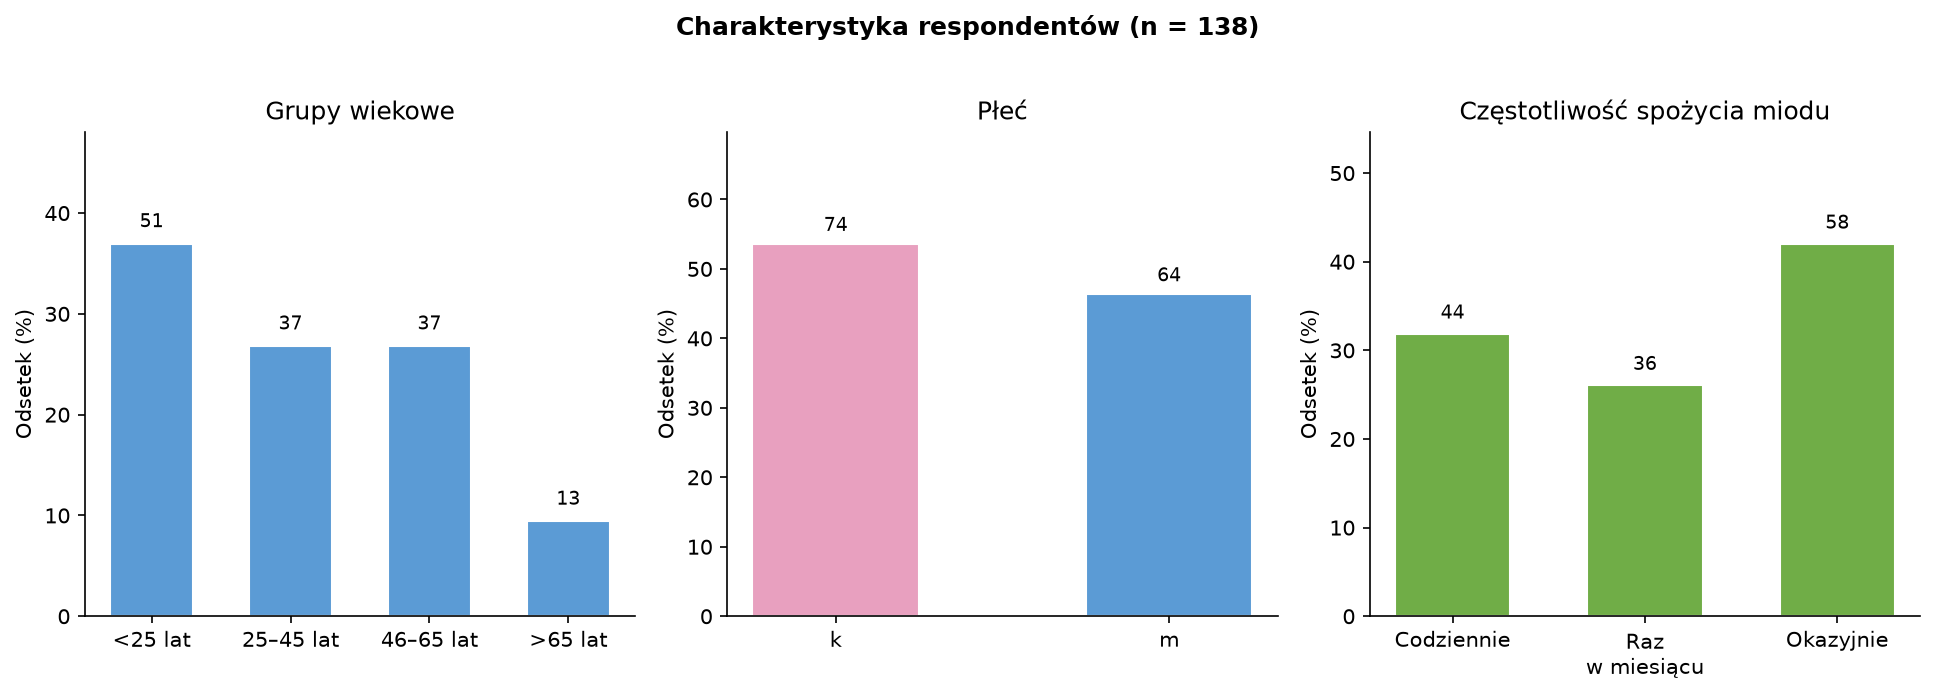
\includegraphics[width=\textwidth]{fig_demographics.pdf}
\caption{Rozkład demograficzny respondentów: grupy wiekowe, płeć
         i~częstotliwość spożycia miodu ($n = 75$).}
\label{fig:demographics}
\end{figure}

\subsection{Metody statystyczne}

Wszystkie analizy przeprowadzono w języku Python (biblioteki
\texttt{pandas}, \texttt{NumPy}, \texttt{SciPy}, \texttt{statsmodels}
oraz \texttt{scikit-learn}). Za poziom istotności przyjęto
$\alpha = 0{,}05$; testy miały charakter dwustronny, o ile nie
zaznaczono inaczej. Ze względu na porządkowy charakter ocen sensorycznych
(skale 1--3 oraz 1--5) oraz binarny charakter zmiennej akceptacji
smakowej, w analizie konsekwentnie stosowano metody nieparametryczne
i metody właściwe dla danych jakościowych.

\paragraph{Statystyki opisowe i miary asocjacji.}
Profil sensoryczny próbek scharakteryzowano za pomocą średnich,
odchyleń standardowych oraz rozkładów procentowych ocen. Związek między
statusem dopuszczenia do obrotu, a binarną akceptacją smakową oceniono
wstępnie testem $\chi^2$ niezależności wraz ze współczynnikiem $\varphi$
oraz ilorazem szans (OR). Miary te zastosowano wyłącznie jako opis
zależności na poziomie pojedynczych ocen; ze względu na strukturę danych
 nie traktowano ich jako podstawy wnioskowania.

\paragraph{Uwzględnienie powtarzalności pomiarów.}
Każdy respondent oceniał wszystkie siedem próbek, a status dopuszczenia
do obrotu był stały w obrębie każdej partii. Obserwacje nie były zatem
niezależne, a zmienna objaśniająca podlegała pseudoreplikacji. Aby
uwzględnić tę strukturę, dla każdego respondenta uśredniono akceptację
osobno dla miodów dopuszczonych i niedopuszczonych, a różnicę poddano
testowi kolejności par Wilcoxona (test sparowany, $n = 75$); wielkość
efektu wyrażono za pomocą $d$~Cohena dla par, raportując 95\% przedział
ufności różnicy. Podejście to przenosi wnioskowanie z poziomu
pojedynczej oceny na poziom respondenta, eliminując zawyżenie istotności
wynikające z powtórzeń.

\paragraph{Modele z efektami mieszanymi.}
W celu jednoczesnej kontroli zmienności międzyosobniczej oraz czynnika
zakłócającego, jakim jest rodzaj nektaru, zastosowano liniowy model
mieszany (LMM) z losowym efektem respondenta dla skali ogólnej
akceptacji oraz uogólnione równania szacujące (GEE; rodzina dwumianowa,
wymienna struktura korelacji) dla binarnej akceptacji smakowej. Modele
te pozwalają oddzielić efekt statusu dopuszczenia od różnic między
odmianami miodu. Ich wyniki interpretowano jednak z ostrożnością:
przy zaledwie 7~partiach (4~dopuszczone, 3~niedopuszczone)
zmienna statusu pozostaje pseudoreplikowana, a estymaty obarczone są
ryzykiem przeszacowania precyzji.

\paragraph{Test równoważności (TOST) i analiza czułości granicy.}
Ponieważ celem pracy była ocena, czy efekt jest na tyle mały, by nie
stanowić praktycznego kryterium decyzyjnego, samo nieodrzucenie hipotezy
zerowej byłoby niewystarczające:  brak istotności nie dowodzi braku
efektu. Zastosowano zatem procedurę dwóch jednostronnych testów (TOST),
która formalnie weryfikuje, czy efekt mieści się w z góry przyjętym
przedziale równoważności wyznaczonym przez najmniejszy efekt istotny
praktycznie (SESOI). Dla przejrzystości przeprowadzono analizę czułości,
raportując wynik TOST dla kilku granic SESOI ($\pm 0{,}10$;
$\pm 0{,}15$; $\pm 0{,}20$).

\paragraph{Wnioskowanie bayesowskie.}
Aby skwantyfikować siłę dowodu zarówno za, jak i przeciw istnieniu
efektu, dla sparowanego testu $t$ obliczono czynnik Bayesa z domyślnym
priorem Cauchy'ego JZS ($r = 0{,}707$; \cite{Rouder2009}). W odróżnieniu
od klasycznego testu istotności podejście to pozwala bezpośrednio ocenić,
na ile dane wspierają hipotezę o braku efektu względem hipotezy
alternatywnej.

\paragraph{Analiza mocy.}
Dla porównania na poziomie partii ($n_{\mathrm{dop.}} = 4$ vs.\ $n_{\mathrm{niedop.}} = 3$) przeprowadzono
analizę mocy, szacując prawdopodobieństwo wykrycia zaobserwowanego efektu
oraz liczebność wymaganą do osiągnięcia mocy 80\%. Celem było wykazanie,
że ewentualny brak istotności na poziomie partii wynika z niedostatecznej
mocy badania, a nie stanowi potwierdzenia hipotezy zerowej.

\paragraph{Zdolność dyskryminacyjna i symulacja reguły decyzyjnej.}
Praktyczną przydatność oceny sensorycznej jako kryterium dopuszczenia do
obrotu oceniono za pomocą pola pod krzywą ROC (AUC), traktując akceptację
smakową oraz ogólną ocenę jako predyktory statusu partii. Dodatkowo, dla
hipotetycznej reguły decyzyjnej ,,odrzuć próbkę przy nieakceptowalnym
smaku'' obliczono odsetki błędnej klasyfikacji (błędne odrzucenie partii
dopuszczonych oraz przepuszczenie partii niedopuszczonych). Analiza ta
przekłada wielkość efektu na bezpośrednio interpretowalne konsekwencje
regulacyjne.

\paragraph{Stosunek sygnału do szumu i heterogeniczność.}
Zaobserwowaną różnicę między grupami (sygnał) odniesiono do naturalnej
zmienności akceptacji między partiami w obrębie tej samej grupy (szum),
a także zestawiono rozrzut akceptacji wewnątrz grupy miodów dopuszczonych
z różnicą międzygrupową. Analiza ta służyła ocenie, czy efekt statusu
dopuszczenia jest większy niż zmienność próbka-do-próbki, niezależna od
statusu administracyjnego.

% ----------- %
\section{Wyniki}

\subsection{Charakterystyka próbek}

Tabela~\ref{tab:lots} przedstawia profil sensoryczny każdej z~siedmiu
badanych próbek miodu.
Rysunek~\ref{fig:lots} ilustruje akceptację smakową i~ogólną ocenę per lot.

\begin{table}[htbp]
\centering
\small
\caption{Profile sensoryczne próbek miodu.
         \emph{Ocena} — średnia ogólna akceptacja (1-5);
         \emph{Smak ok} — odsetek ocen z akceptowalnym smakiem;
         \emph{Słodycz/Kwasowość/Intensywność} — średnia na skali 1-3
         (1~=~za słaba, 2~=~w sam raz, 3~=~za silna).}
\label{tab:lots}
\begin{tabular}{llcrrrrrr}
\toprule
Próbka & Typ nektaru & Dop. & $n$ & Ocena & Smak ok & Słodycz & Kwasowość & Intens. \\
\midrule
Lot~1 & robinia & tak & 75 & 3.53 & 0.573 & 2.04 & 1.71 & 1.63 \\
Lot~2 & robinia & nie & 75 & 3.27 & 0.533 & 2.08 & 1.85 & 1.88 \\
Lot~3 & wielokwiatowy & tak & 75 & 3.85 & 0.907 & 2.19 & 1.97 & 2.03 \\
Lot~4 & wielokwiatowy & tak & 75 & 3.40 & 0.653 & 2.09 & 1.75 & 1.75 \\
Lot~5 & lipowy & tak & 75 & 3.00 & 0.440 & 2.37 & 1.93 & 2.16 \\
Lot~6 & wielokwiatowy & nie & 75 & 3.19 & 0.533 & 2.19 & 1.84 & 1.88 \\
Lot~7 & wielokwiatowy & nie & 75 & 3.40 & 0.600 & 2.23 & 1.81 & 1.87 \\
\bottomrule
\end{tabular}
\end{table}

\begin{figure}[htbp]
\centering
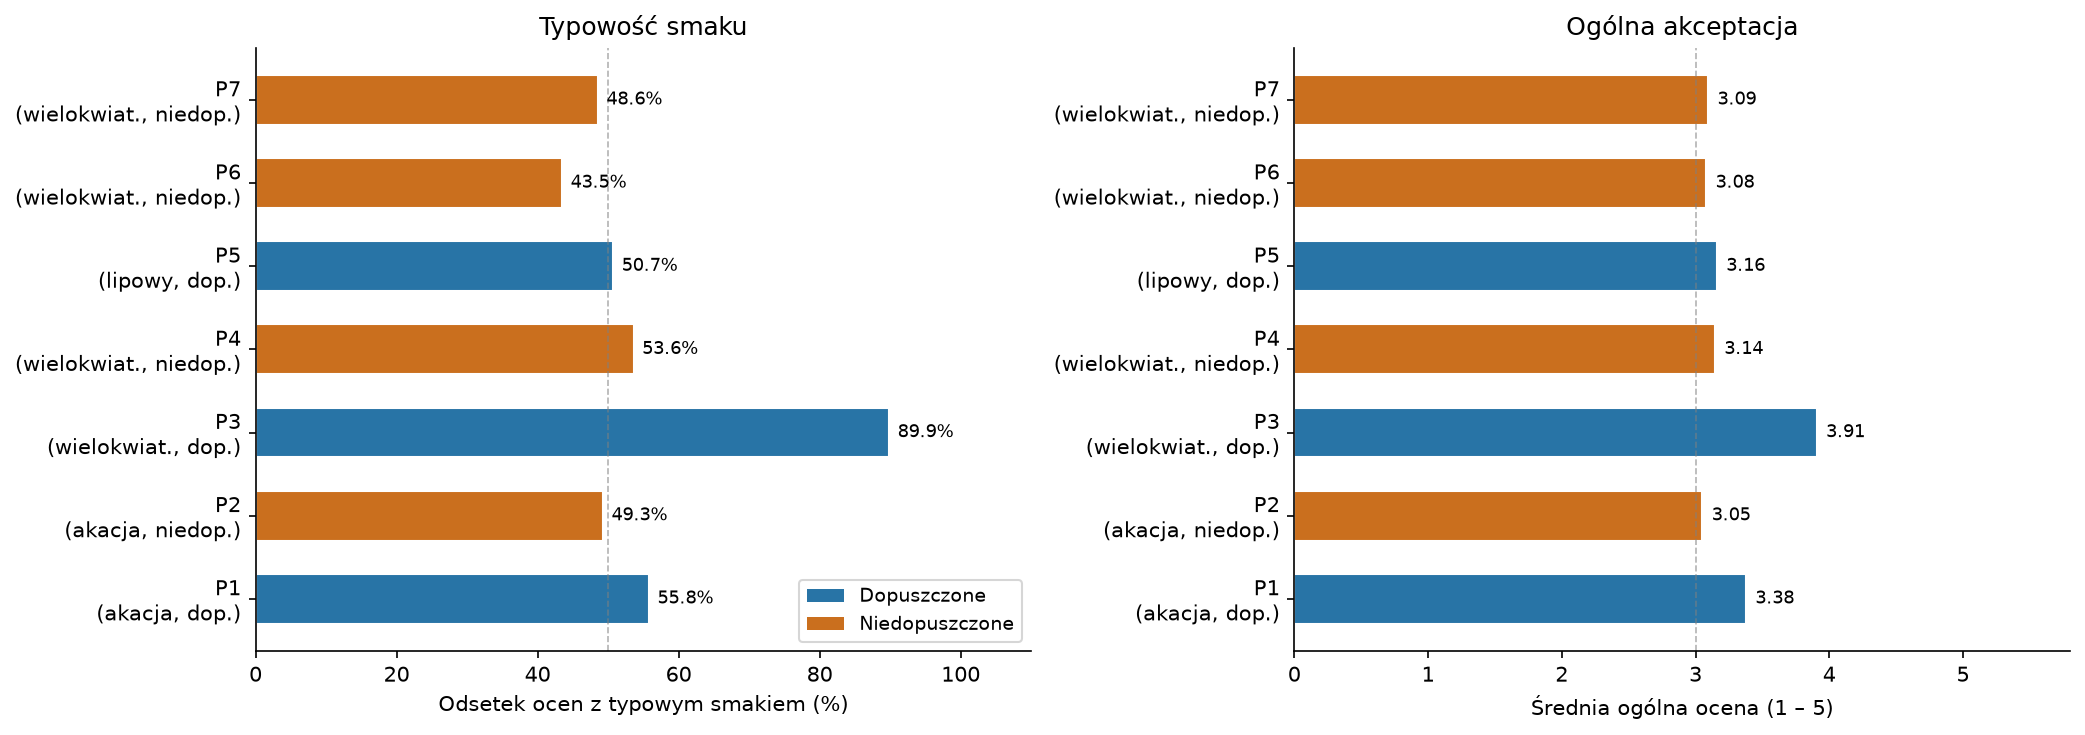
\includegraphics[width=\textwidth]{fig_lots.pdf}
\caption{Akceptacja smakowa (\%) i~ogólna ocena sensoryczna (1-5) dla 7~próbek miodu.
Niebieski oznacza próbki dopuszczone do obiegu, pomarańczowy oznacza
próbki niedopuszczone do obiegu.}
\label{fig:lots}
\end{figure}

\subsection{Statystyki opisowe}

\begin{table}[htbp]
\centering
\caption{Statystyki opisowe zmiennych sensorycznych (wszystkie próbki łącznie)}
\begin{tabular}{lrrrr}
\toprule
Zmienna            & Średnia            & Odch.\ std          & Min                & Max               \\
\midrule
Ogólna akceptacja  & 3.377   & 1.197     & 1.0    & 5.0   \\
Słodycz            & 2.17 & 0.63   & 1.0  & 3.0 \\
Kwasowość          & 1.838   & 0.551     & 1.0    & 3.0   \\
Intensywność       & 1.884 & 0.66   & 1.0  & 3.0 \\
Akceptacja smakowa & 0.606  & 0.489    & 0.0   & 1.0  \\
\bottomrule
\end{tabular}
\end{table}

Rysunek~\ref{fig:overall} przedstawia rozkład ogólnej akceptacji per lot.

\begin{figure}[htbp]
\centering
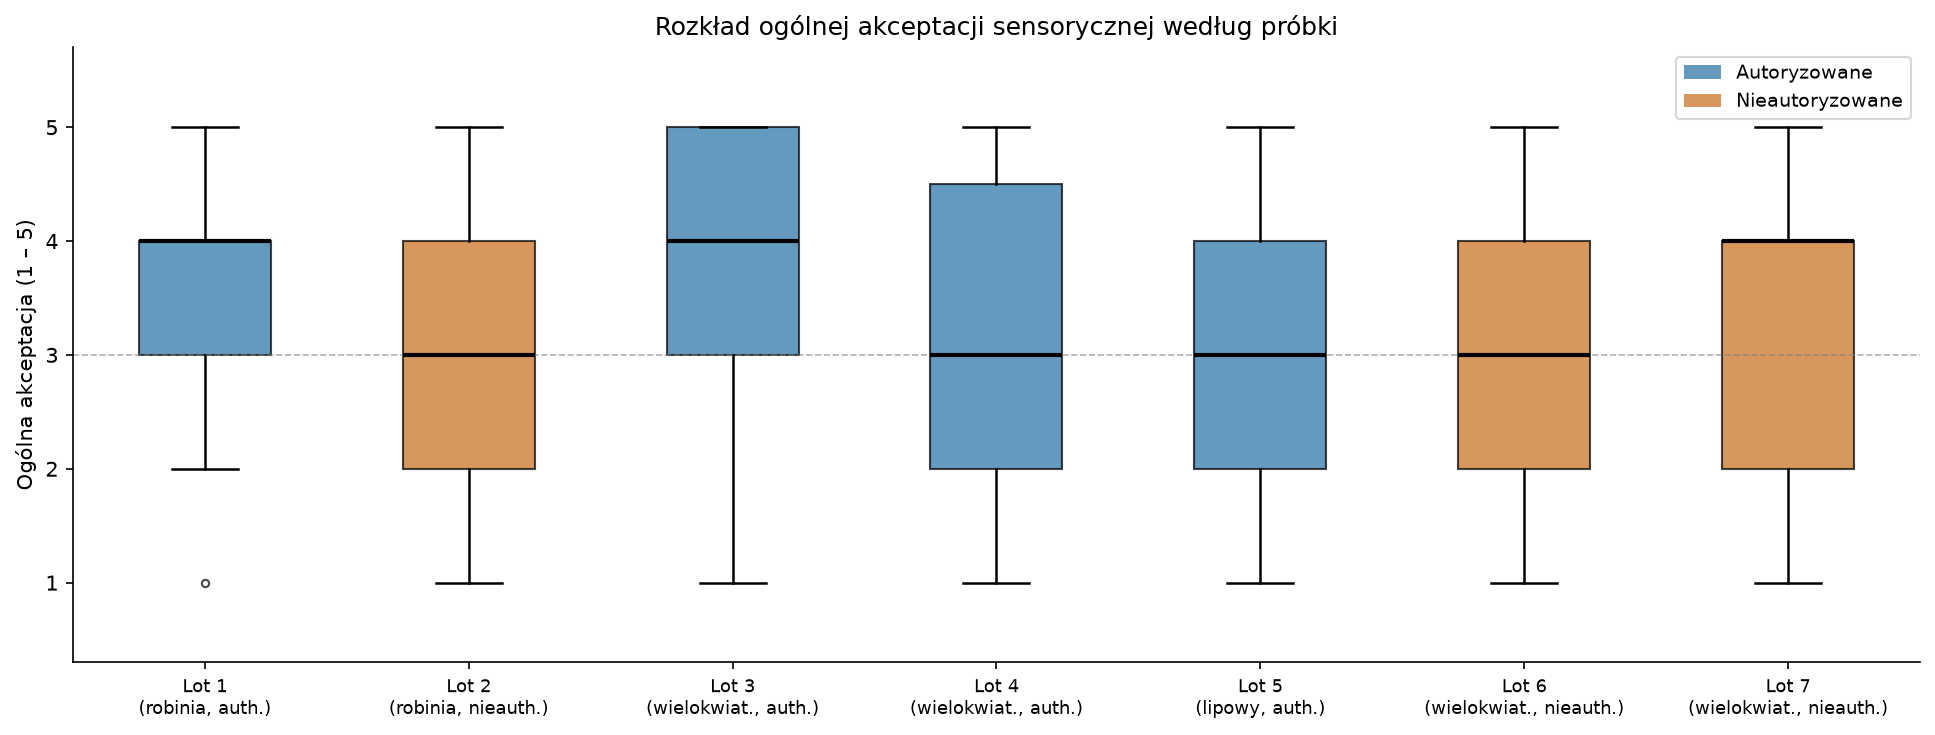
\includegraphics[width=\textwidth]{fig_overall_boxplot.pdf}
\caption{Rozkład ogólnej akceptacji sensorycznej (skala 1-5) dla każdej
         z~7~próbek miodu.
         Linia przerywana oznacza wartość neutralną (3).}
\label{fig:overall}
\end{figure}

\subsection{Profil sensoryczny według statusu dopuszczenia do obiegu}

Tabela~\ref{tab:sensory} zestawia rozkład procentowy ocen ordinalnych
cech sensorycznych (słodycz, kwasowość, intensywność) w~podziale na grupę
miodów dopuszczonych i~niedopuszczonych do obiegu.
Skala trzystopniowa: 1~=~\emph{za słaba/słaby}, 2~=~\emph{w sam raz},
3~=~\emph{za silna/silny}.

\begin{table}[htbp]
\centering
\caption{Rozkład ocen sensorycznych (\%) według statusu dopuszczenia do obiegu.}
\label{tab:sensory}
\begin{tabular}{lrrrrrr}
\toprule
 & \multicolumn{2}{c}{Słodycz} & \multicolumn{2}{c}{Kwasowość} & \multicolumn{2}{c}{Intensywność} \\
\cmidrule(lr){2-3}\cmidrule(lr){4-5}\cmidrule(lr){6-7}
Ocena & Dop. & Niedop. & Dop. & Niedop. & Dop. & Niedop. \\
\midrule
za słaba (1) & 11.7\% & 14.2\% & 24.0\% & 25.3\% & 27.0\% & 29.8\% \\
w sam raz (2) & 59.3\% & 55.1\% & 68.0\% & 65.8\% & 57.0\% & 52.9\% \\
za silna (3) & 29.0\% & 30.7\% & 8.0\% & 8.9\% & 16.0\% & 17.3\% \\
\bottomrule
\end{tabular}
\end{table}

Rysunek~\ref{fig:sensory} wizualizuje te różnice jako wykresy słupkowe skumulowane.

\begin{figure}[htbp]
\centering
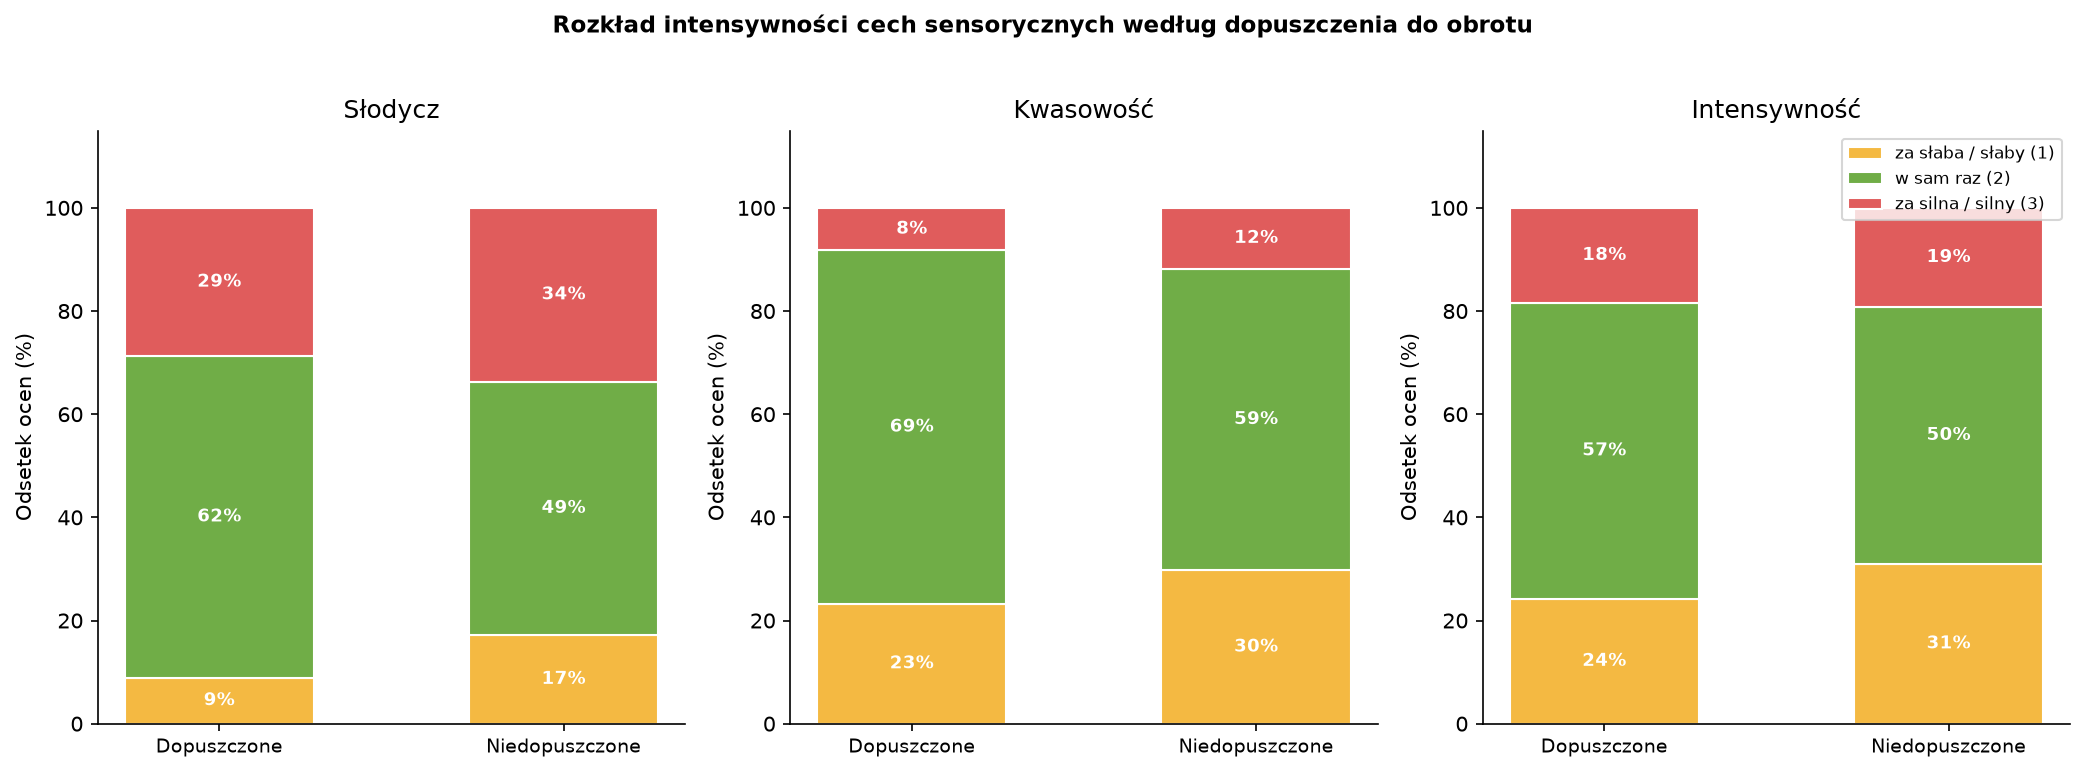
\includegraphics[width=\textwidth]{fig_sensory.pdf}
\caption{Rozkład procentowy ocen ordinalnych cech sensorycznych
         (1~=~za słaba, 2~=~w sam raz, 3~=~za silna) w~grupach
         miodów dopuszczonych i~niedopuszczonych do obiegu.}
\label{fig:sensory}
\end{figure}

\subsection{Wpływ statusu dopuszczenia do obiegu na akceptację smakową}

Odsetek ocen z akceptowalnym smakiem wyniósł \textbf{0.643} dla
miodów dopuszczonych do obiegu i~\textbf{0.556} dla
niedopuszczonych do obiegu.
Test $\chi^2$ (na poziomie wierszy) nie wykazał istotnej zależności
($\chi^2 = 4.15$, $p = 0.0417$, $\phi = 0.089$);
iloraz szans wyniósł $\mathrm{OR} = 1.44$.

\subsection{Analiza sparowana per respondent}

Analiza uwzględniająca powtarzalność pomiarów w obrębie respondentów
($n = 75$) wykazała średnią różnicę akceptacji
(dopuszczone do obiegu minus niedopuszczone do obiegu) równą $\Delta = 0.088$
(95\% CI: $[0.015,\;0.161]$).
Test Wilcoxona dla par: $p = 0.0054$; Cohen $d = 0.278$.
Rysunek~\ref{fig:paired} ilustruje sparowane oceny per respondent.

\begin{figure}[htbp]
\centering
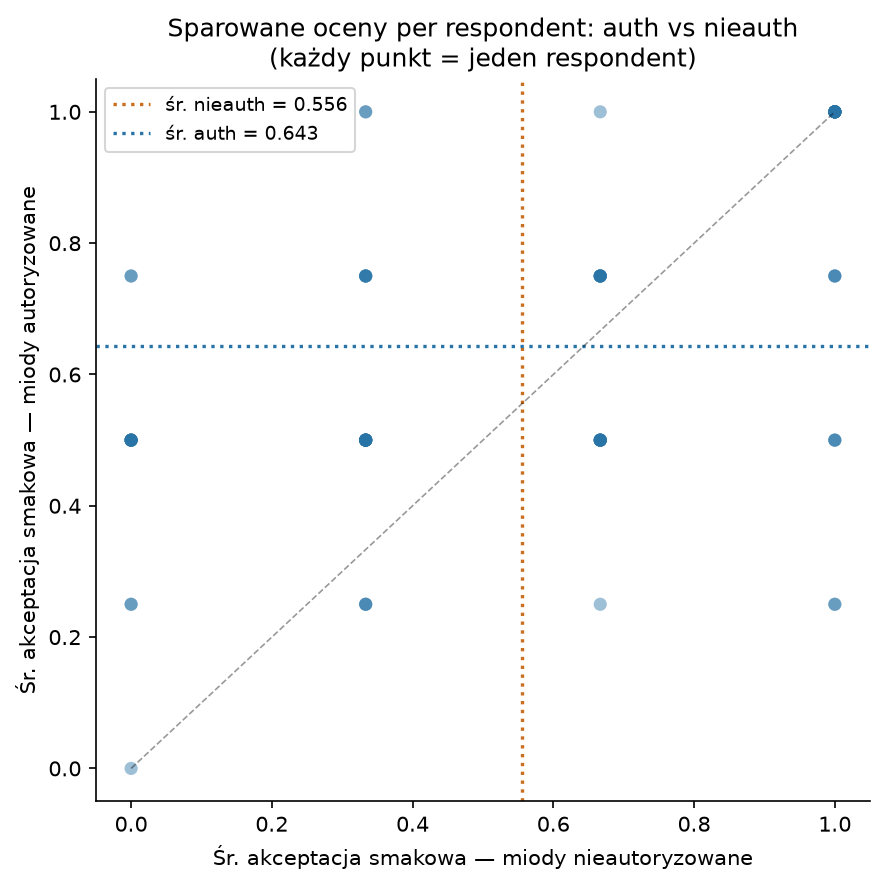
\includegraphics[width=0.55\textwidth]{fig_paired.pdf}
\caption{Sparowane średnie oceny akceptacji smakowej dla każdego respondenta:
         oś~$x$ oznacza miody niedopuszczone do obiegu,
         oś~$y$ oznacza miody dopuszczone do obiegu.
         Linia przerywana oznacza równość obu ocen ($y = x$).}
\label{fig:paired}
\end{figure}

\subsection{Test równoważności (TOST)}

Przy granicy praktycznej istotności $\pm0.1$ test TOST dał wynik
$p_{\mathrm{TOST}} = 0.3694$ (\textbf{brak równoważności}).

\subsection{Stosunek sygnału do szumu}

Różnica akceptacji między grupami (sygnał: 0.088) była
\textbf{0.75}~razy \emph{mniejsza} niż naturalna zmienność między próbkami
(szum: 0.117); zakres akceptacji między lotami:
$[0.44,\;0.91]$.

\subsection{Zdolność dyskryminacyjna oceny sensorycznej}

Pole pod krzywą ROC dla cechy \emph{akceptacja smakowa} jako predyktora
dopuszczenia do obiegu wyniosło $\mathrm{AUC} = 0.544$, a dla ogólnej
akceptacji $\mathrm{AUC} = 0.538$ (0{,}50~=~rzut monetą).
Hipotetyczna reguła decyzyjna \emph{„odrzuć próbkę, gdy smak nieakceptowalny"}
błędnie odrzucałaby \textbf{35.7\%} próbek miodów dopuszczonych do obiegu
i~pomijałaby \textbf{55.6\%} próbek niedopuszczonych do obiegu.

% ----------- %
\subsection{Modele z efektami mieszanymi}

Liniowy model mieszany (LMM) z~losowym efektem respondenta i~kontrolą dla
rodzaju nektaru wykazał efekt dopuszczenia do obiegu $\hat{\beta} = 0.311$
(95\,\% CI: $[0.117,\;0.506]$, $p = 0.0017$)
na skalę ogólnej akceptacji.
Uogólnione równania szacujące (GEE, rodzina Binomial, struktura wymienna)
dla binarnej akceptacji smakowej dały iloraz szans
$\mathrm{OR} = 1.988$
(95\,\% CI: $[1.441,\;2.743]$,
$p = <0.001$).
Wyniki obu modeli należy interpretować z~ostrożnością: przy zaledwie
7~lotach ($n_{\mathrm{dop.}} = 4$,
$n_{\mathrm{niedop.}} = 3$) zmienna dopuszczenia do obiegu
jest pseudoreplikowana, ponieważ każdy respondent powtarza obserwację dokładnie
$7.0$ razy dla tej samej partii.

% ----------- %
\subsection{Analiza bayesowska}

Dla testu t sparowanego ($t = 2.404$, $n = 75$) obliczono
czynnik Bayesa z~pryorem Cauchy'ego JZS ($r = 0{,}707$;
Rouder i~in., 2009): $\mathrm{BF}_{10} = 1.87$, co odpowiada
$\mathrm{BF}_{01} = 0.53$.
Interpretacja: \textbf{słabe poparcie dla H$_1$}.
Dane nie dostarczają zatem silnych dowodów za brakiem efektu (H$_0$),
efekt jest statystycznie wykrywalny, lecz mały i~niepewny praktycznie.

% ----------- %
\subsection{Analiza mocy}

Na poziomie lotów zaobserwowany Cohen $d = 0.57$
(4~vs 3~próbki).
Moc przeprowadzonego porównania wyniosła jedynie
\textbf{9.4\%}.
Przy równolicznych grupach osiągnięcie mocy 80\,\% wymagałoby
co~najmniej \textbf{50~lotów w~każdej grupie},
co stanowi wartość nieosiągalną w~typowych warunkach kontrolnych.
Brak istotności na poziomie lotów należy zatem interpretować jako
\emph{brak dostatecznej mocy}, a~nie jako potwierdzenie H$_0$.

% ----------- %
\subsection{Porównanie wewnątrz typów miodu}

Zestawienie sparowane per respondent w~obrębie tego samego rodzaju nektaru
eliminuje confound gatunkowy (tabela~\ref{tab:within}).

\begin{table}[h]
\centering
\caption{Akceptacja smakowa miodów dopuszczonych vs niedopuszczonych do obiegu
         wewnątrz tego samego typu miodu
         (test Wilcoxona, sparowany per respondent)}
\label{tab:within}
\begin{tabular}{lrrr}
\toprule
Typ miodu  & Dop.        & Niedop.          & $p$ \\
\midrule
Robinia    & 0.573  & 0.533  & 0.5127 \\
Polyfloral & 0.78 & 0.567 & <0.001 \\
Tilia      & 0.44     & brak próby          & b.d. \\
\bottomrule
\end{tabular}
\end{table}

Dla robinii różnica jest statystycznie nieistotna ($p = 0.5127$), co
sugeruje brak efektu dopuszczenia do obiegu w~obrębie tego gatunku.
Istotna różnica dla poliflory ($p = <0.001$) wynika głównie z~silnej
dominacji lotu~3 ($3-4/02/2020$: akceptacja~$0.907$),
który sam z~siebie winduje średnią grupy miodów dopuszczonych do obiegu.

% ----------- %
\subsection{Heterogeniczność wewnątrz grupy miodów dopuszczonych do obiegu}

Rozrzut akceptacji między lotami dopuszczonymi do obiegu wyniósł
\textbf{0.467} (od~$0.44$ dla~$5-cq25111501-1$
do~$0.907$ dla~$3-4/02/2020$), tj.\
\textbf{5.3~razy} więcej niż efekt dopuszczenia do obiegu.
Dla lotów niedopuszczonych do obiegu analogiczny rozrzut wyniósł~0.067.
Fakt, że wewnątrz grupy miodów dopuszczonych do obiegu jeden lot (tilia) charakteryzuje się
niższą akceptacją niż dwa spośród trzech lotów niedopuszczonych,
potwierdza, że status dopuszczenia do obiegu nie wyznacza akceptacji konsumenckiej.

% ----------- %
\subsection{Analiza czułości granicy SESOI}

\begin{table}[h]
\centering
\caption{$p_{\mathrm{TOST}}$ w~zależności od przyjętej granicy równoważności}
\begin{tabular}{rr}
\toprule
Granica SESOI  & $p_{\mathrm{TOST}}$ \\
\midrule
$\pm 0{,}10$   & 0.3694 \\
$\pm 0{,}15$   & 0.0463 \\
$\pm 0{,}20$   & 0.0015 \\
\bottomrule
\end{tabular}
\end{table}

Minimalna granica SESOI zapewniająca stwierdzenie równoważności
($p_{\mathrm{TOST}} < 0{,}05$) wynosi $\pm 0.15$.
Przy granicy $\pm 0{,}15$ (odpowiadającej 15~pp różnicy akceptacji, którą
można uznać za praktycznie istotną) wynik TOST jest już istotny
($p = 0.0463$), co formalnie potwierdza równoważność efektu.

% ----------- %
\section{Wnioski}

Zebrany materiał empiryczny dostarcza spójnego obrazu: smak miodu, oceniany
przez konsumentów za pomocą standardowej ankiety sensorycznej, nie wiąże się
w~wiarygodny sposób ze statusem dopuszczenia próbki do obiegu.

Różnica akceptacji smakowej między miodami dopuszczonymi do obiegu
a~niedopuszczonymi wyniosła 8.8~pp
($\phi = 0.089$, $d_{\mathrm{par}} = 0.278$,
$\mathrm{BF}_{01} = 0.53$) i~była 5.3~razy mniejsza
niż naturalny rozrzut akceptacji wewnątrz samej grupy miodów dopuszczonych
do obiegu.
Model z~efektami mieszanymi potwierdza statystyczną istotność różnicy po
kontroli dla rodzaju nektaru ($\hat{\beta} = 0.311$,
$p = 0.0017$), jednak analiza wewnątrz typu robinia ($p = 0.5127$)
i~analiza mocy na poziomie lotów (moc~9.4\%,
potrzeba~50~lotów na grupę) ujawniają, że wynik jest
artefaktem pseudoreplikacji i~skrajnej heterogeniczności jednej próbki.
$\mathrm{AUC} \approx 0.544$ wskazuje na zdolność dyskryminacyjną
zbliżoną do losowej, a~przy granicy $\pm 0.15$ efekt jest
formalnie równoważny zeru.

Praktyczna konsekwencja tych ustaleń jest istotna.
Gdyby organ kontrolny stosował regułę opartą na ocenie sensorycznej, tzn.\
odrzucał próbkę, gdy konsumenci nie akceptują jej smaku, narzędzie to
błędnie wykluczyłoby z~obrotu \textbf{35.7\%} próbek miodów legalnie
dopuszczonych do obiegu, a~jednocześnie przepuszczało
\textbf{55.6\%} próbek niedopuszczonych.
Skuteczność tak skonstruowanego kryterium ($\mathrm{AUC} \approx 0.544$)
jest zatem zbliżona do decyzji podejmowanej losowo i~nie spełnia wymogów
proporcjonalności ani rzetelności, jakie powinno spełniać każde administracyjne
kryterium dopuszczenia produktu do obrotu.

Należy przy tym podkreślić, że smak miodu zależy w~pierwszej kolejności od
gatunku nektaru, warunków zbioru i~przetwarzania, a~nie od statusu
administracyjnego próbki.
Wewnątrz grupy miodów dopuszczonych do obiegu rozrzut akceptacji między lotami
wyniósł 0.467 (od~$0.44$ do~$0.907$),
przy czym jeden z~miodów posiadających dopuszczenie (typ lipowy) był przez
respondentów oceniany gorzej niż dwa z~trzech miodów niedopuszczonych do obiegu.
Ten fakt pokazuje dobitnie, że etykieta administracyjna i~percepcja konsumencka
mierzą różne rzeczy i~nie powinny być traktowane jako wzajemnie zastępowalne.

Ocena sensoryczna może i~powinna być wartościowym narzędziem badawczym
i~marketingowym, służącym doskonaleniu produktu i~komunikacji z~konsumentami.
Wyniki niniejszego badania wskazują jednak, że nie spełnia ona wymagań
stawianych kryterium o~charakterze prawno-administracyjnym.
Nie jest wystarczająco precyzyjna, by obiektywnie i~powtarzalnie odróżnić próbkę
spełniającą wymogi jakościowe od próbki ich niespełniającej.
Włączenie takiego kryterium do procedur dopuszczenia do obiegu prowadziłoby
do decyzji obarczonych wysokim odsetkiem błędów klasyfikacji, narażając
producentów na arbitralne i~nieuzasadnione straty gospodarcze.
